% Template for IGARSS-2018 paper; to be used with:
%          spconf.sty  - LaTeX style file, and
%          IEEEbib.bst - IEEE bibliography style file.
% --------------------------------------------------------------------------
\documentclass{article}
\usepackage{spconf,amsmath,epsfig}
\usepackage[hidelinks]{hyperref}
\usepackage{etoolbox}
\usepackage{textcomp}
% Example definitions.
% --------------------
\def\x{{\mathbf x}}
\def\L{{\cal L}}

% Title.
% ------
\title{FRESH SNOW DEPTH ESTIMATION USING SPACEBORNE X-BAND POLARIMETRIC SYNTHETIC APERTURE RADAR DATA}
%
% Single address.
% ---------------
\name{Sayantan Majumdar\textsuperscript{1,2}, Praveen K. Thakur\textsuperscript{3}, Ling Chang\textsuperscript{1}, Shashi Kumar\textsuperscript{4}}
\address{\textsuperscript{1}Department of Earth Observation Science, Faculty of Geo-information Science and Earth Observation\\ (ITC), University of Twente, Enschede, The Netherlands\\
\textsuperscript{2}Geoinformatics Department, Indian Institute of Remote Sensing (IIRS), ISRO, Dehradun, India\\
\textsuperscript{3}Water Resources Department, Indian Institute of Remote Sensing (IIRS), ISRO, Dehradun, India \\
\textsuperscript{4}Photogrammetry and Remote Sensing Department, Indian Institute of Remote Sensing (IIRS), ISRO,\\ Dehradun, India\\
Email: \href{mailto: sayantan.majumdar@ieee.org}{sayantan.majumdar@ieee.org}, \href{mailto: praveen@iirs.gov.in}{praveen@iirs.gov.in}, \href{mailto: ling.chang@utwente.nl}{ling.chang@utwente.nl}, \href{mailto: shashi@iirs.gov.in}{shashi@iirs.gov.in} 
}
\tolerance=1
\emergencystretch=\maxdimen
\hyphenpenalty=10000
\hbadness=10000
\sloppy

\begin{document}
%\ninept
%
\maketitle
%
\begin{abstract}
The estimation of fresh snow depth (FSD) using X-band synthetic aperture radar (SAR) is feasible but challenging depending on the geological conditions and data availability. In this study, the FSD is computed for the Beas river watershed in the northwestern Himalayas near Manali, India. It incorporates the recent copolar phase difference (CPD) based FSD inversion model. Moreover, the TerraSAR-X and TANDEM-X bistatic data acquired in January 2016 are used as inputs to the model along with the snow density measurements at the Dhundi ground station. Additionally, apart from applying layover and forest masks, the potential uncertainty sources in the complex mountainous terrains are identified using the H-A-$\alpha$ decomposition and unsupervised Wishart classification techniques. Furthermore, due to the limited number of weather stations, the results are validated using a 3x3 neighbourhood window surrounding the Dhundi site. Also, the effect of different FSD ensemble window sizes are tested for performing sensitivity analysis.
\end{abstract}
%
\begin{keywords}
Fresh snow, synthetic aperture radar, copolar phase difference, polarimetry, snow anisotropy
\end{keywords}
%
\section{Introduction}
\label{sec:intro}
Snow depth or snow height is one of the most important physical properties of snow and finds extensive usage in hydrological models, particularly in snowmelt runoff and snow avalanche predictions \cite{Thakur2012}. Essentially, it represents the height of the snow surface from the ground underneath. Moreover, it is also used to measure the snow water equivalent (SWE) which quantifies the amount of water present in a snowpack \cite{Tedesco2015}. However, accurate snow depth estimation can be challenging depending on the availability of suitable data and the geological situations of the study area \cite{Leinss2014}, \cite{Leinss2015}.

In this regard, standard practice is to couple remote sensing techniques with adequately sampled spatiotemporal ground observations, thereby improving the quality of the resultant snow depth map \cite{Thakur2012}, \cite{Leinss2014}, \cite{Leinss2015}. Nowadays, Light Detection and Ranging (LiDAR) and Synthetic Aperture Radar (SAR) have been widely adopted for measuring snow depth with sufficiently high accuracies in the order of centimetres \cite{Tedesco2015}, \cite{Leinss2014}, \cite{Deems2013}. Although laser altimetry measurements offer high-quality results, the data acquisition is sensitive to weather conditions and is also expensive \cite{Deems2013}. Therefore, spaceborne SAR, which facilitates globally available high-resolution datasets along with weather independency and night-time operability, is extensively utilised in the cryospheric studies \cite{Thakur2012}, \cite{Leinss2014}, \cite{Moreira2013}.

Since snow is a porous birefringent medium which is a mixture of air, ice and water, the microwave interactions occurring at all these constituent phases need to be properly understood. For frequencies X-band and below, the major backscattering occurs at the snow-ground interface in case of dry snow, whereas surface scattering contributes the maximum when the snow is wet. However, humid snow exhibits a significant volume scattering which occurs within the snowpack \cite{Thakur2012}, \cite{Leinss2014}. In essence, the scattering mechanism is governed by the volumetric liquid water content of the snowpack which is responsible for controlling the microwave absorption in snow \cite{Leinss2014}.

In addition to this, the snow metamorphism induced anisotropy and snow density are critical factors which must be considered for estimating the fresh snow depth (FSD). X-Ray computer tomography scans have shown that in the initial stage, the freshly fallen snow exhibits a random structure which upon settling is transformed to horizontally aligned or oblate particles having snow densities in the range of 0.03-0.12 g/cm\textsuperscript{3}. Gradually, vertically shaped prolate particles (firn and depth hoar) are formed displaying snow density values in the order of 0.5 g/cm\textsuperscript{3}. After further recrystallisation, solid ice is produced whose density has been found to be 0.917 g/cm\textsuperscript{3} \cite{Leinss2014}, \cite{Riche2013}. Moreover, the effective permittivity ($\epsilon_{snow}$) of dry snow (fresh snow, firn, and depth hoar) is independent of the microwave frequency in the 10 MHz to 1 THz electromagnetic (EM) wave spectrum and only shows a strong dependence on the snow density \cite{Leinss2015}.

In principle, the three orthogonal axes ($a_x$, $a_y$, $a_z$) of a spheroid represented in the 3D ($x$, $y$, $z$) Cartesian coordinate system correspond to the three dipoles which essentially characterises the dielectric nature of an ice particle. This is highlighted in figure \ref{fig:prolate}, where a prolate ice particle is linked with the radar reference frame ($h$, $k$, $v$) following the radar backscattering alignment (BSA) convention. Here, $k$, $h$ and $v$ are the propagation vector, wave components of the horizontal and vertical polarisations respectively, $\theta$ being the satellite incidence angle obtained with respect to the surface normal \cite{Leinss2014}.

\AfterEndEnvironment{figure}{\vspace{-1ex}}
\begin{figure}[htb]
\centering
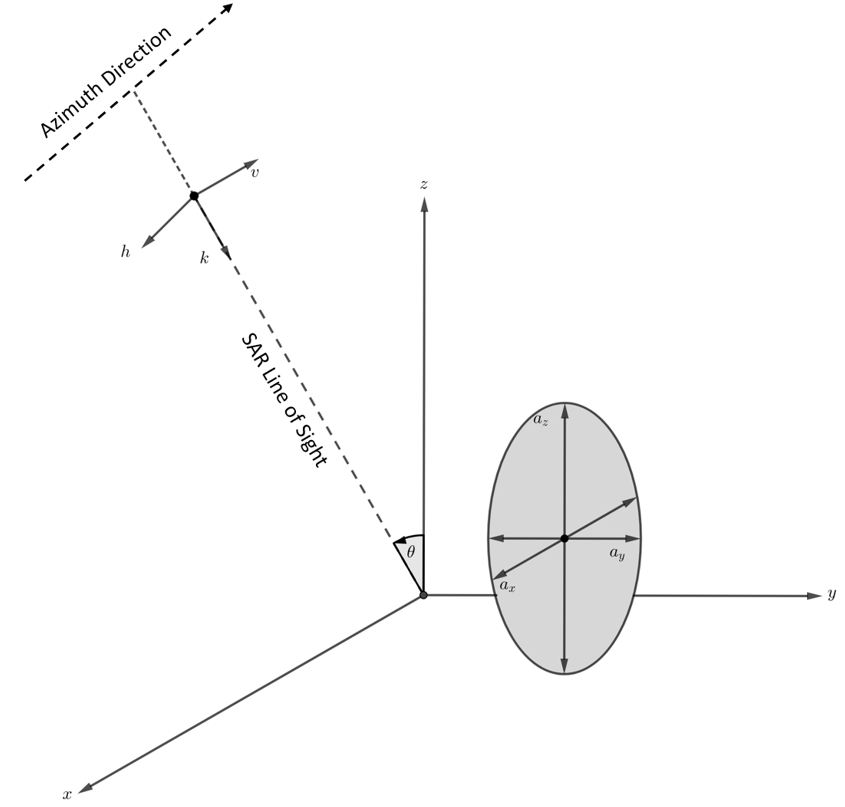
\includegraphics[scale=0.2]{Prolate_New.png}
\caption{The orientation of a single prolate ice particle linked with the radar reference frame (adapted from \cite{Leinss2014}).}
\label{fig:prolate}
\end{figure}

Furthermore, the depolarisation factor is an important component to model the snow anisotropy which in turn, is used as a parameter in the FSD inversion algorithm based on the copolar phase difference (CPD) approach \cite{Leinss2014}. In this work, the CPD method is applied to compute the FSD in the complex alpine terrains of the Beas watershed, northwestern Himalayas. Additionally, due to the extreme geological conditions there exist significant uncertainty sources which are discussed explicitly in the later sections.

\section{Study area and Data}
\label{sec:study}
\subsection{Study Area}
\label{ssec:area}
The Beas river watershed near Manali, India is characterised by steep slopes and dense forests. The elevation varies from about 2500 m to more than 5000 m (figure \ref{fig:overview}). In this work, the Beas basin, starting from a few kilometres uphill from Dhundi up to Kothi (figure \ref{fig:overview}) has been chosen for FSD estimation. The areas surrounding Dhundi and Kothi receive significant seasonal snowfall usually from the onset of December to late March. However, the cold, dry season starts from as early as October. The coldest period is in January with temperatures reaching a mean daily minimum of -15\textsuperscript{0}C whereas, in June, mean and maximum temperatures of 20\textsuperscript{0}C and 30\textsuperscript{0}C respectively are commonly observed. Additionally, heavy rainfall occurs in the monsoon season (late June-September) with August being the wettest month \cite{Thakur2012}. In total, an area of approximately 130 km\textsuperscript{2} is depicted in Figure \ref{fig:overview} showing ALOS PALSAR digital elevation model (DEM). Here, the original 12.5 m DEM has been resampled to 3 m to match the high-resolution SAR data used in this research. 

\AfterEndEnvironment{figure}{\vspace{-3.5ex}}
\begin{figure}[htb]
\centering
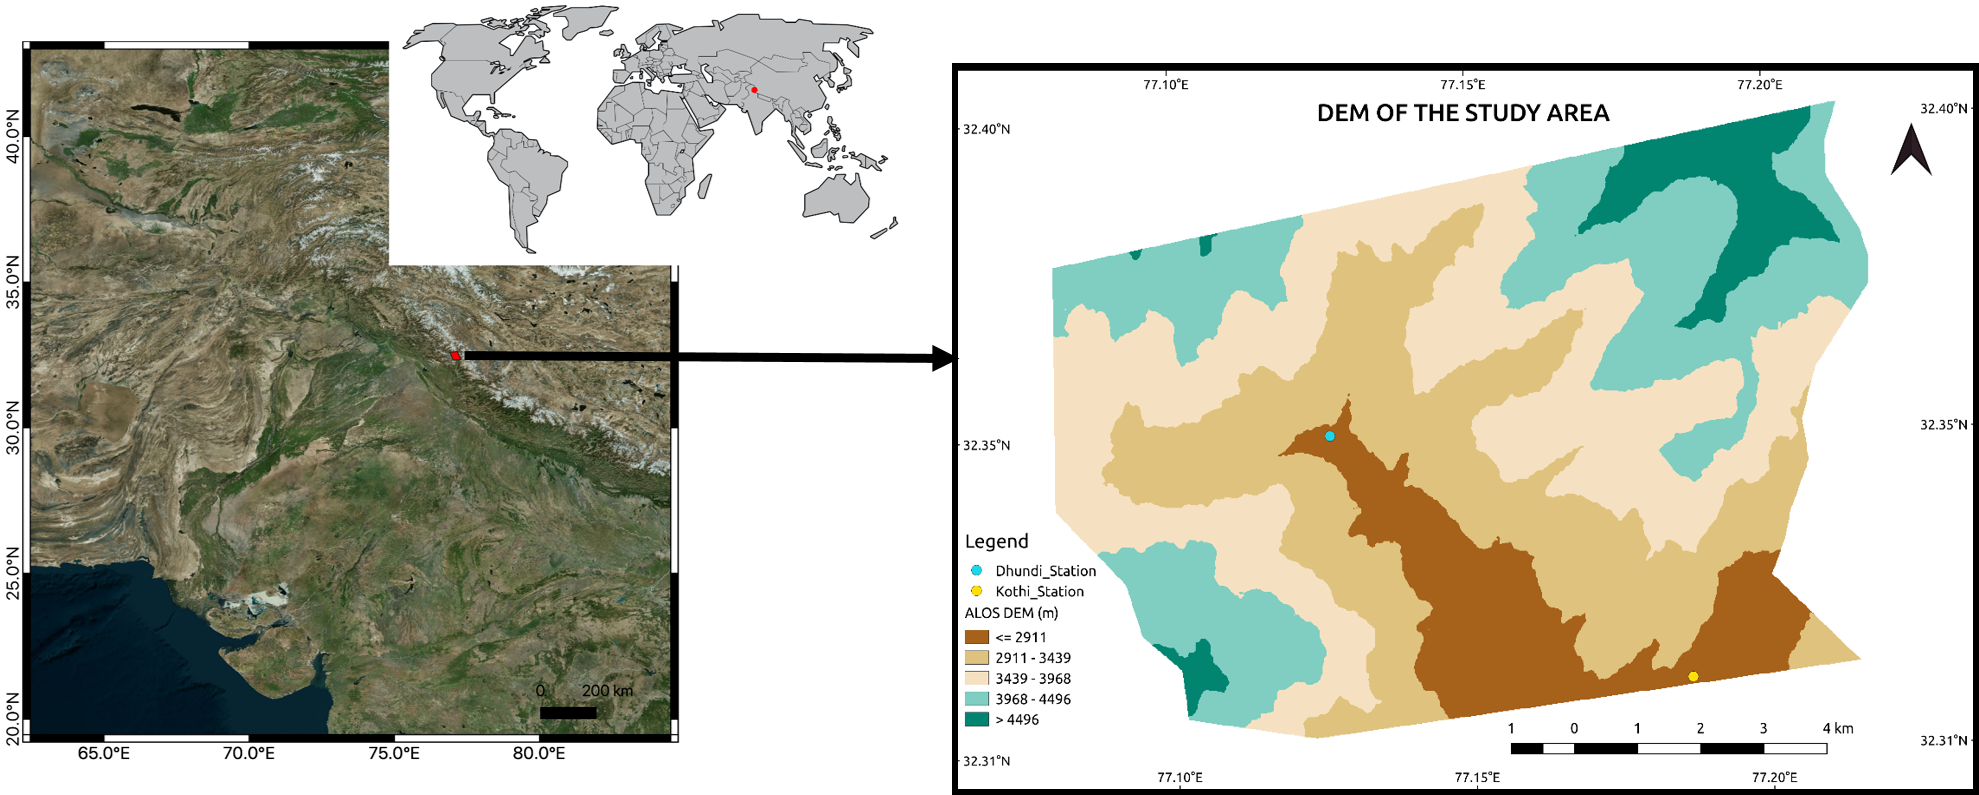
\includegraphics[width=7.5cm]{Overview.png}
\caption{The overview map of the study area showing the ALOS PALSAR DEM, Dhundi and Kothi ground stations.}
\label{fig:overview}
\end{figure}

\subsection{Available Datasets}
\label{ssec:data}
Regarding the SAR data, fully polarimetric (Quad-pol) and Coregistered Single look Slant range Complex (CoSSC) X-band bistatic acquisitions in stripmap (SM) mode from TerraSAR-X and TANDEM-X satellites have been used. Overall six Quad-pol data pairs were available, out of which the descending orbital pass acquisition at 00:53 hrs, Jan 8, 2016, has been selected considering the occurrence of fresh snowfall before, during and after the satellite flyby.

Additionally, intensive fieldwork had been conducted from Oct 14-21, 2018 in the Dhundi and Kothi areas where several differential GPS (DGPS) measurements were acquired with adequate positional accuracies ($\sim$7 cm). Moreover, the in-situ snow physical parameters’ data (total and fresh snow depths, snow density) along with the relevant weather data were transferred to a PostgreSQL database from the manual recordings. Accordingly, the fresh snow depths on the Jan 7, 2016 evening and Jan 8, 2016 morning were 5 cm and 22 cm respectively signifying a heavy snowfall event.

Apart from this, a Landsat 8 OLI acquisition over the study area on May 12, 2016 (summer season) had been downloaded to prepare the forest mask.    


\vspace{-1ex}
\section{Methodology}
\label{sec:method}
The steps involved in this research workflow are depicted in figure \ref{fig:work}. All the processing tasks have been carried out using open-source tools and libraries which include the Sentinel Application Platform (SNAP), QGIS and Python.

At first, the CoSSC product has been split into separate TerraSAR-X, and TANDEM-X images and then radiometric calibration has been applied. After subsetting these images, the CPDs are computed individually using \eqref{1} where $\Im$ and $\Re$ denote the imaginary and real parts of the complex scattering matrices $S_{VV}$ and $S_{HH}$ respectively ($\phi_{VV}$ and $\phi_{HH}$ representing the corresponding phases), $\langle\rangle$ denoting the ensemble averaging operation. These are subsequently averaged to a single CPD image. Thereafter, terrain correction is performed using the ALOS PALSAR DEM where the local incidence angle (LIA) is also stored as an image band alongside CPD.
\AfterEndEnvironment{figure}{\vspace{4ex}}
\begin{figure}[htb]
\centering
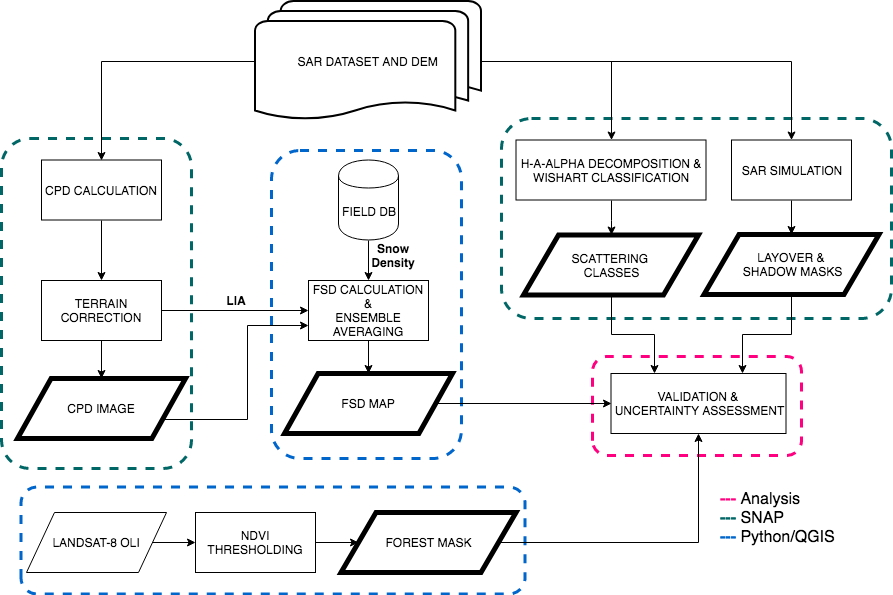
\includegraphics[scale=0.248]{Method_FSD.png}
\caption{The research workflow highlighting the major tasks.}
\label{fig:work}
\end{figure}

The geocoded CPD image (3 m spatial resolution) is then used as an input to the FSD estimation module written in Python. Initially, the CPD values are averaged based on an ensemble window of 21x21 pixels (4 km\textsuperscript{2} ground area). The FSD ($\Delta Z_f$) inversion model is given by \eqref{2} where the CPD ($\phi_{CPD}\in[-\pi,\pi]$), radar wavelength ($\lambda_0$), LIA ($\theta_l$), and the two snow refractive indices, $n_V$ and $n_H$ (corresponding to the two polarisations VV and HH respectively) are the involved parameters. In this regard, it has been found that for fresh snow,  $\phi_{CPD}>0$ and $n_H>n_V$, i.e., $\Delta{\zeta}<1$ \cite{Leinss2014}. Essentially, \eqref{2} is based on the underlying Maxwell-Garnett EM mixture model and the depolarisation factor equations, a detailed treatment of which is provided by \cite{Sihvola1999}. The estimated FSD values are further averaged using different square and rectangular ensemble windows after which the final map is prepared in QGIS.
\vspace{-1.9ex}
\begin{center}
    \vspace{-1.9ex}
    \begin{equation}\tag{1}
        \small{\phi_{CPD} =\left\langle\underbrace{tan^{-1}\left(\frac{\Im\left(S_{VV}\right)}{\Re\left(S_{VV}\right)}\right)}_{\phi_{VV}} - \underbrace{\tan^{-1}\left(\frac{\Im\left(S_{HH}\right)}{\Re\left(S_{HH}\right)}\right)}_{\phi_{HH}}\right\rangle}
        \label{1}
    \end{equation}
    \begin{equation}\tag{2}
        \small{\Delta{Z_f} = (-1)\frac{\lambda_0\phi_{CPD}}{4\pi\Delta{\zeta}}}
        \label{2}
    \end{equation}
    \centering
    where $\small{\Delta{\zeta} = \sqrt{n^2_V - \sin^{2}\theta_l} - \sqrt{n^2_H - \sin^{2}\theta_l}}$
\end{center}

Additionally, layover, shadow (SAR simulation) and forest masks (NDVI thresholding) are generated (3 m spatial resolution) to assess the potential uncertainty sources qualitatively. Moreover, the H-A-$\alpha$ decomposition and unsupervised Wishart classification techniques have been used to compare the scattering mechanisms in the study sites during snow-covered (Jan 8, 2016) and snow-free (Jun 8, 2016) seasons \cite{Singh2014}.     

\section{Results and Discussion}
\label{sec:results}

To achieve the best rendering in the proceedings, we
strongly encourage you to use Times-Roman font.  In addition, this will give
the proceedings a more uniform look.  Use a font that is no smaller than nine
point type throughout the paper, including figure captions.

In nine point type font, capital letters are 2 mm high.  If you use the
smallest point size, there should be no more than 3.2 lines/cm (8 lines/inch)
vertically.  This is a minimum spacing; 2.75 lines/cm (7 lines/inch) will make
the paper much more readable.  Larger type sizes require correspondingly larger
vertical spacing.  Please do not double-space your paper.  True-Type 1 fonts
are preferred.

The first paragraph in each section should not be indented, but all the
following paragraphs within the section should be indented as these paragraphs
demonstrate.

\section{Conclusion}
\label{sec:concl}

Major headings, for example, "1. Introduction", should appear in all capital
letters, bold face if possible, centered in the column, with one blank line
before, and one blank line after. Use a period (".") after the heading number,
not a colon.



% References should be produced using the bibtex program from suitable
% BiBTeX files (here: strings, refs, manuals). The IEEEbib.bst bibliography
% style file from IEEE produces unsorted bibliography list.
% -------------------------------------------------------------------------
\bibliographystyle{IEEEbib}
\bibliography{IEEEabrv,refs}

\end{document}
